% 1350 words
\section*{}
To recapitulate our findings thus far: First, we have established that provided with open data on population, amenity points-of-interest density and diversity, and public transportation accessibility indices, we can predict the total number of arrivals by public transport to a high degree of accuracy using an XGBoost machine learning model that is fine-tuned to overcome overfitting and converge fast. Secondly, we extracted more sophisticated feature importance indications using SHAP for machine learning model explanation than originally achievable with the XGBoost model's internal tree-path structure. Thirdly, the methodology allows us to decompose each target variable (i.e., arrivals by public transport) prediction into the sum of each feature's contribution in the form of its SHAP value.in effect, by examining local SHAP values' spatial distributions, we can identify hotspots for different POI features overall and across different time bands.

One of the benefits of using SHAP values as imperfect approximants to coefficients in a statistical model is their additive nature. This means that we can decompose the model's predictions into the sum of the SHAP values, with which we can control for unwanted effects. For example, without an explicit origin-destination matrix and dwell time data and using only station exits and bus alighting data, it is not immediately possible to say whether a person is exiting at a destination to attend an activity or to interchange to another mode of transport. Using SHAP to extract local explanations with its additive property, therefore, can help isolate the impact of the amenity profile of the destination area on the trip attractiveness of the area while controlling for the contribution of its connectivity profile based on how well the model predicts the total arrivals for each spatial unit.

\begin{figure}[!htb]
    \centering
    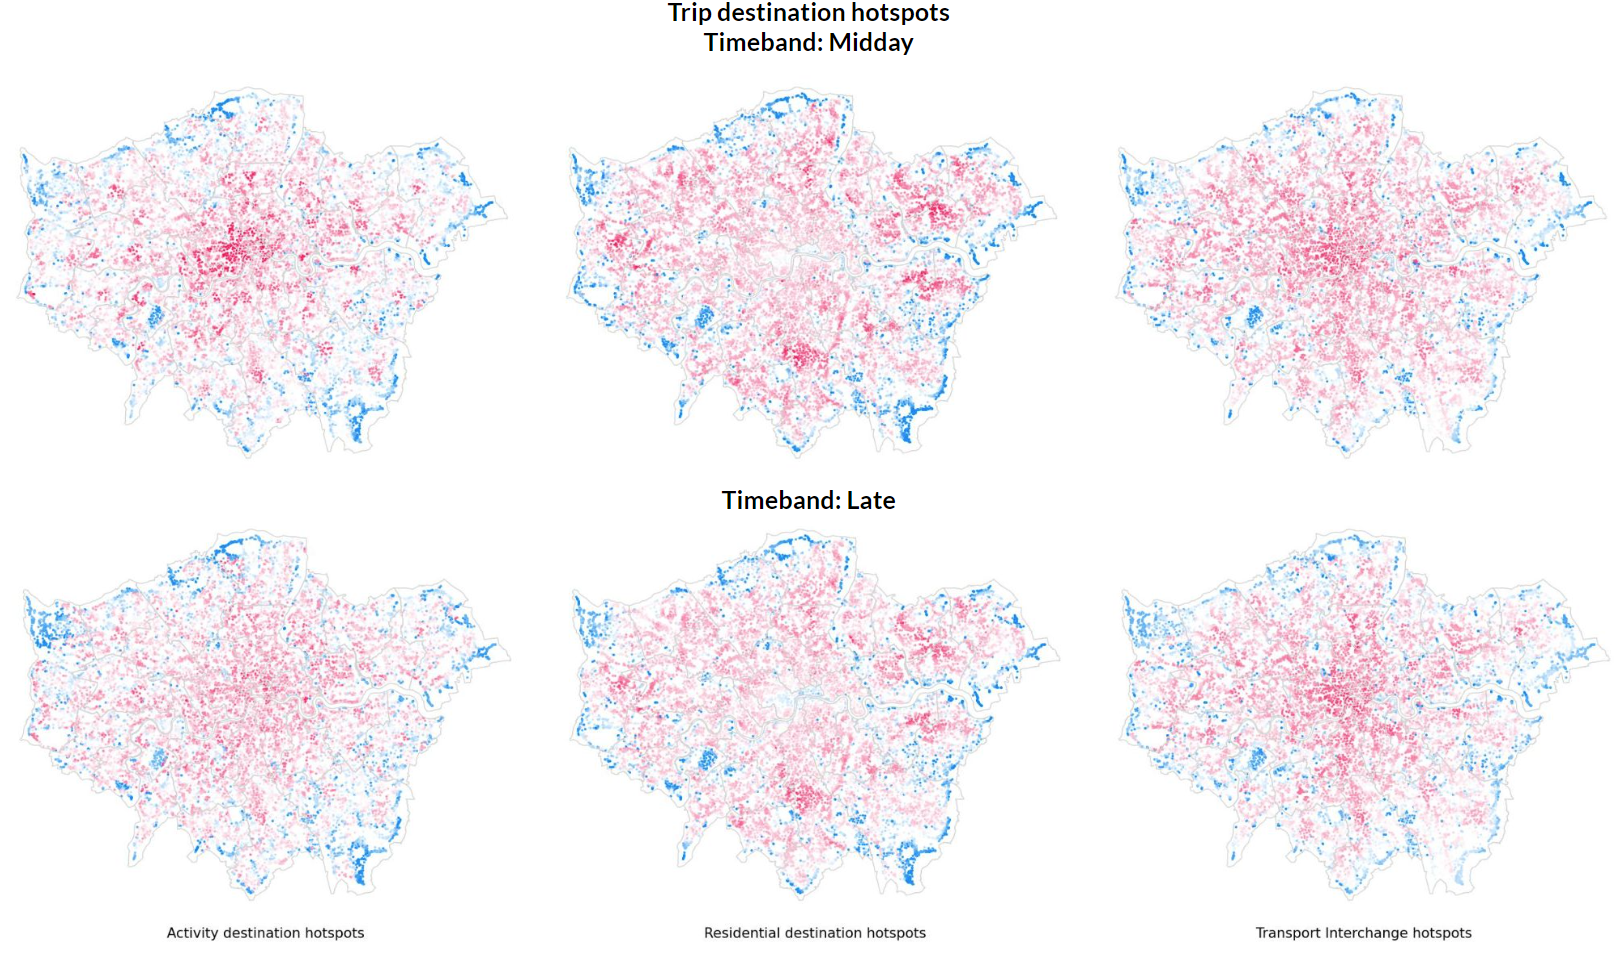
\includegraphics[width=\textwidth]{destinationhotspot.png}
    \captionsetup{justification=centering}
    \caption{Amenity vs. Residential vs. Transit "Hotspots" \\Calculated as the sum of SHAP values for each feature group in each spatial unit\\Timeband: Midday vs. Late}
    \label{fig:destinationhotspot}
\end{figure}

One way to visualise it is by grouping local SHAP values by feature groups and visualising their spatial distribution. This can be seen in Figure \ref{fig:destinationhotspot} with our 25 features grouped into (1) all 13 amenity-related features, (2) population feature, and (3) all 11 connectivity-related features. When comparing the Midday and Late time bands, representing the peak and lowest volumes, respectively, we can see that the impact of the amenity profile on trip attractiveness is significantly more pronounced in the Midday time band, whereas the impact of the connectivity profile on trip attractiveness is seemingly unchanged (i.e., they have visually similar spatial distributions). Since we can assume that the connectivity-related features in our model (density of transport nodes, centrality measures, etc.) are static and independent of time bands\footnote{Service scheduling and frequency of public transport services are not considered in our model}, and that the only difference between these two time bands is the trip attraction generated by amenities, this suggests that the model can isolate whether an area attracts trip because of the presence of the amenities. This is insightful for instances where we want to qualify whether certain areas are urban activity hotspots based on the availability of amenities while excluding demand generated with the purpose of interchange for onward journeys (i.e., "transit" hotspots). 

\pagebreak
\noindent This can be summarised via a generalised formula for Activity Hotspot Index

$$A_i = \sum_{j} h_{ij}$$

\noindent where $A_i$ is the Activity Hotspot Index of spatial unit $i$ and $h_{ij}$ is the local SHAP value of amenity-related feature $j$ of spatial unit $i$\footnote{In total, there are 15 density-based amenity features and 1 amenity diversity feature. See the Methodology chapter for further clarifications.}. Applying spatial clustering such as HDBSCAN on the isochrones based on spatial units' Activity Hotspot Index $A$ effectively surfaces activity hotspots in Greater London, as shown in Figure \ref{fig:activityhotpost} with the top 10\% activity hotspots based on the mean activity hotspot index of all member spatial units. These hotspots are areas where the amenity profile has the highest mean SHAP values across all spatial units in the cluster, indicating that these areas are popular for non-commute activities based on the amenity profile of the area. Figure \ref{fig:woodgreen} demonstrates a closer look at Wood Green's top activity hotspot cluster, comprised of five member spatial units (isochrones). This can be useful for local urban planners to identify destination areas that are popular for non-commute activities, such as parks, shopping, dining, or entertainment.

\begin{figure}
    \centering
    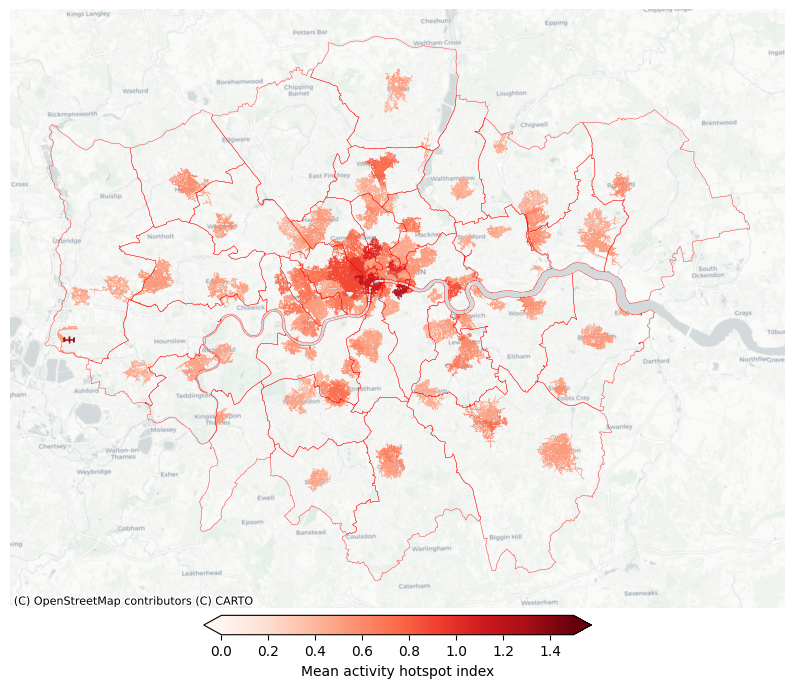
\includegraphics[width=0.8\textwidth]{activityhotspot.png}
    \captionsetup{justification=centering}
    \caption{Top 10\% activity hotspot clusters in Greater London\\Based on mean activity hotspot index of member spatial units}
    \label{fig:activityhotpost}
\end{figure}

\begin{figure}[!hbt]
    \centering
    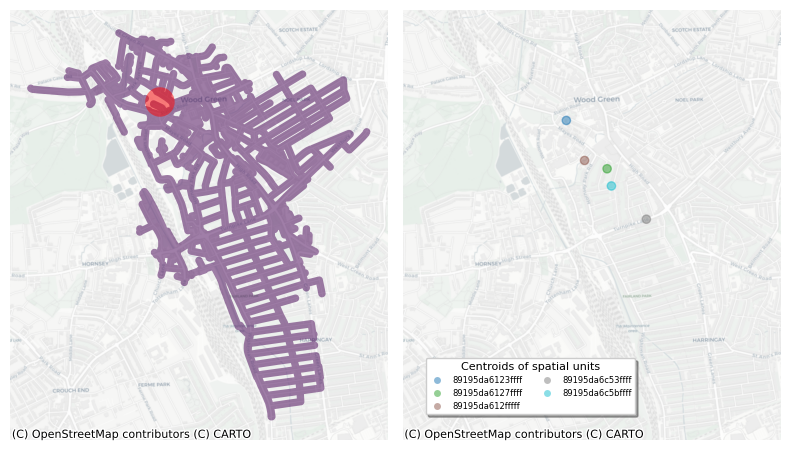
\includegraphics[width=0.8\textwidth]{woodgreen.png}
    \captionsetup{justification=centering}
    \caption{Top activity hotspot cluster in Wood Green by mean Activity Hotspot Index (left) and the centroids of the five member spatial units (right)}
    \label{fig:woodgreen}
\end{figure}

In summary, by using SHAP explanations for an XGBoost model's predictions of total arrivals in an area in Greater London based on ts amenity and connectivity features, we can uncover spatial and temporal patterns of urban activities, and identify destination hotspots for different purposes, such as activities tied to different urban amenities or transit interchange. The dissertation's findings are summarised in Figure \ref{fig:summary}.

\pagebreak
Finally, it is worth acknowledging the methodology's limitations, which affect its generalisability and applicability in some instances.

\begin{itemize}
    \setlength\itemsep{0em}
    \item \textit{Core assumptions in the selection of target variables}: In order to approximate non-commute trip attractiveness, we opted for data on a Saturday as a typical weekend day to remove the effect of employment centres from the analysis as much as possible. However, this does not account for travel demand from those who work on weekends. Future work could consider using a more comprehensive dataset that includes trip purpose information to better understand the non-commute trip attractiveness of an area if such distinction is essential for the analysis. 
    \item \textit{Missing features}: The analysis of outliers suggests that other factors may influence the number of arrivals in an area not accounted for in the model. These could include socioeconomic factors, car ownership, or other urban morphological features that affect people's usage of public transport. Incorporating these features into the model could improve its accuracy and generalisability in localities with high variance in public transport usage.
    \item \textit{Generalisability}: The high feature importance of the spatial lag features across the board means that the model may not accurately predict a new observation in isolation from its neighbours, nor can it be readily generalisable to other cities. Nevertheless, the model can predict the trip attractiveness of a given area in Greater London as the city changes, giving transport planners a useful tool. For example, when a neighbourhood is undergoing redevelopment, we can predict the potential inflow of public transport trips based on the planned addition of amenities or transport facilities and connectivity.
    \item \textit{POI classification}: The classification of amenity and transport POIs in this analysis adheres to Geofabrik's out-of-the-box OSM data classification. Future work could attempt to reclassify these POIs more deliberately to capture the association between certain trip purposes of interest and the types of amenities that fulfil them as destinations.
    \item \textit{Quality of open data}: More broadly, due to the reliance on open data as part of the methodology, the data quality used in the analysis is subject to the quality of the data sources. Varying degrees of quality in the open data available across different localities, especially OSM data, could lead to incorrect predictions and conclusions. 
\end{itemize}

The dissertation scope is also limited to public transport trips and does not account for other types of urban mobility, such as cycling, walking, ridesharing, or driving, which would provide a more comprehensive understanding of the non-commute trip attractiveness of an area regardless of mode of transport, especially during time bands when public transport is less accessible such as late nights. As an extension of this shortcoming, activity hotspots identified so far may only hold true for public transit users. Future work could incorporate mode-agnostic mobility data and trip purpose inferences into a modified version of this methodology to provide a more comprehensive understanding of what draws people to a certain area in Greater London. Special care should be taken to ensure that the connectivity-related features, in this case, reflect the transport modes of interest. For example, to engineer connectivity-related features with active means of transport such as cycling, the density of cycle lanes and bike-sharing stations would be more relevant than the density of bus stops and rail stations.

\begin{figure}[!hbt]
    \centering
    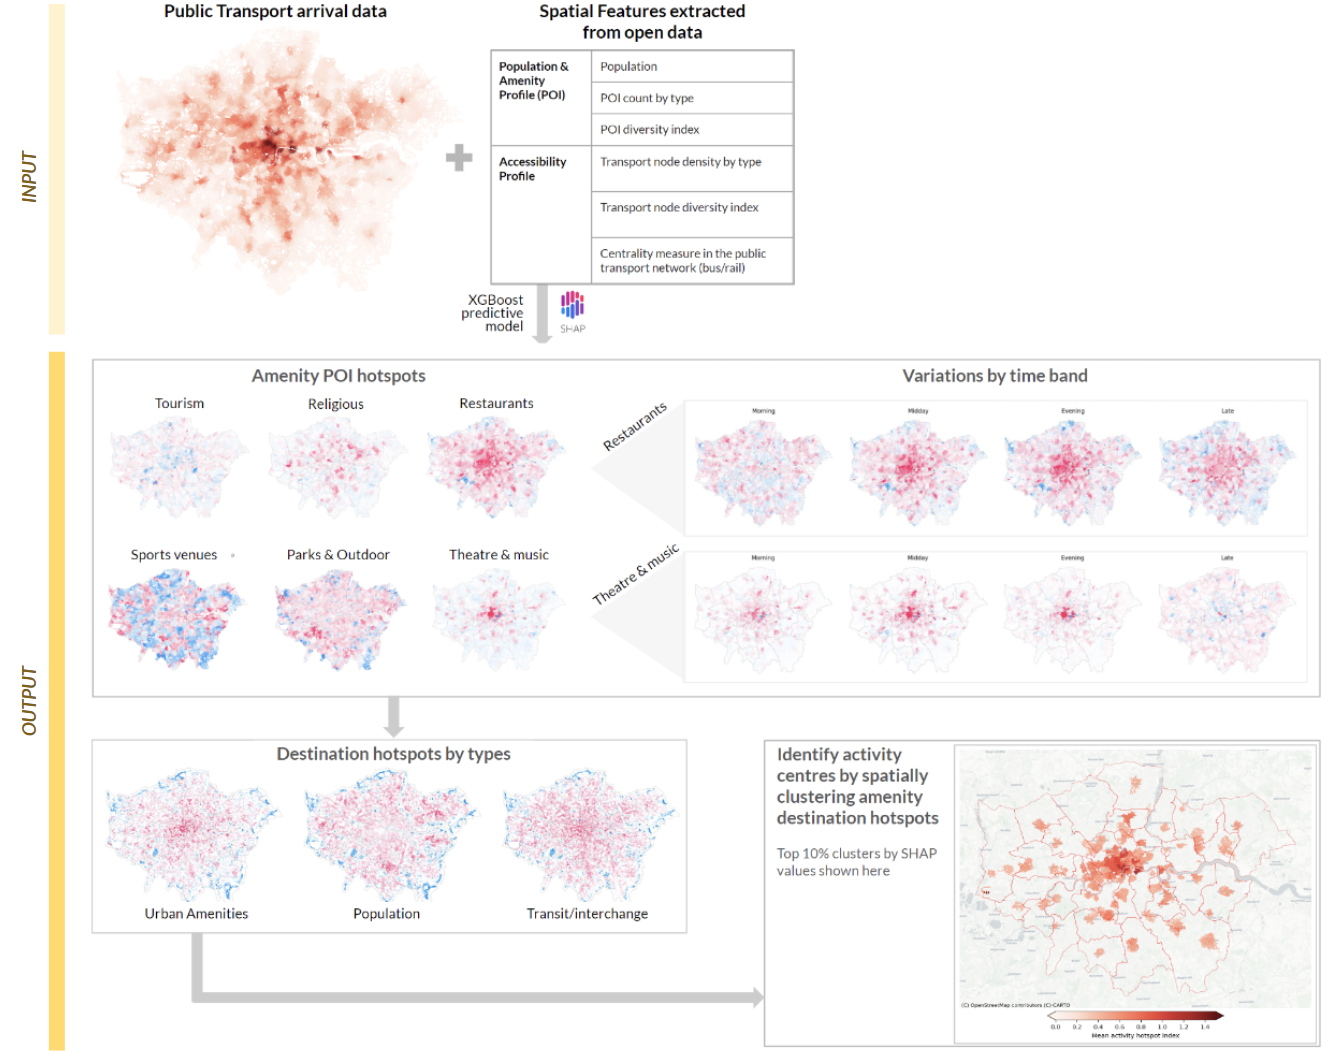
\includegraphics[width=\textwidth]{summary.png}
    \captionsetup{justification=centering}
    \caption{Summary of inputs and outputs (non-exhaustive)\\from the methodology proposed in this study}
    \label{fig:summary}
\end{figure}
